\section{Vorgehen}

\begin{figure}[H]
	\centering
	\includegraphics[height=9cm]{img/vorgehen.png}
	\caption{Übersicht Vorgehen}
	\label{fig:vorgehen}
\end{figure} 

\subsection{DNA Center Initiales Setup}

\subsubsection{Installation}
\label{DNACenterSetup_Installation}
Die Installation des DNA Centers erfolgt direkt an der Konsole oder über die Cisco IMC. Dabei wird die maglev-config-wizard ausgeführt. Dieser Befehl kann im nachhinein jederzeit zur Anpassung der Konfiguration ausgeführt werden. 

Wie in \cite{cisco-dna-installation-guide} Kapitel 2 beschrieben werden folgende Angaben benötigt:
\begin{itemize}
	\item Host IP Adresse
	\item Netmask
	\item Default Gateway IP adress
	\item DNS Servers
	\item Static Routes
	\item HTTPS Proxy
	\item Maglev Mster Node IP
	\item Username, Password und Linux Password
	\item Administration Passphrase (for Web Access)
	\item NTP Servers
	\item Service Subnet
\end{itemize}

Im ersten Schritt \ref{fig:dna-center-install-step-1} wird gewählt, ob ein neues Cluster erstellt werden soll oder einem Beigetreten werden soll. Bei der Testumgebung dieser Arbeit war nur eine Appliance verfügbar, weshalb ausschliesslich "Start a DNA-C Cluster" ausgewählt wurde. 

\begin{figure}[H]
	\centering
	\includegraphics[height=9cm]{img/sc_001.png}
	\caption{DNA Center Configuration Wizard Start}
	\label{fig:dna-center-install-step-1}
\end{figure} 

\begin{figure}[H]
	\centering
	\includegraphics[height=9cm]{img/sc_002.png}
	\caption{DNA Center Configuration Wizard - Entering Management IP}
	\label{fig:dna-center-install-step-4}
\end{figure} 

\begin{figure}[H]
	\centering
	\includegraphics[height=9cm]{img/sc_003.png}
	\caption{DNA Center Configuration Wizard - Entering Authentification Data}
	\label{fig:dna-center-install-step-13}
\end{figure}

\begin{figure}[H]
	\centering
	\includegraphics[height=9cm]{img/sc_004.png}
	\caption{DNA Center Configuration Wizard - DNA Center uses docker}
	\label{fig:dna-center-install-step-install}
\end{figure}


\subsubsection{Setup Accounts}
Nach dem der Wizard die Installation vollständig ausgeführt hat, ist das DNA Center Web-GUI verfügbar.
\begin{figure}[H]
	\centering
	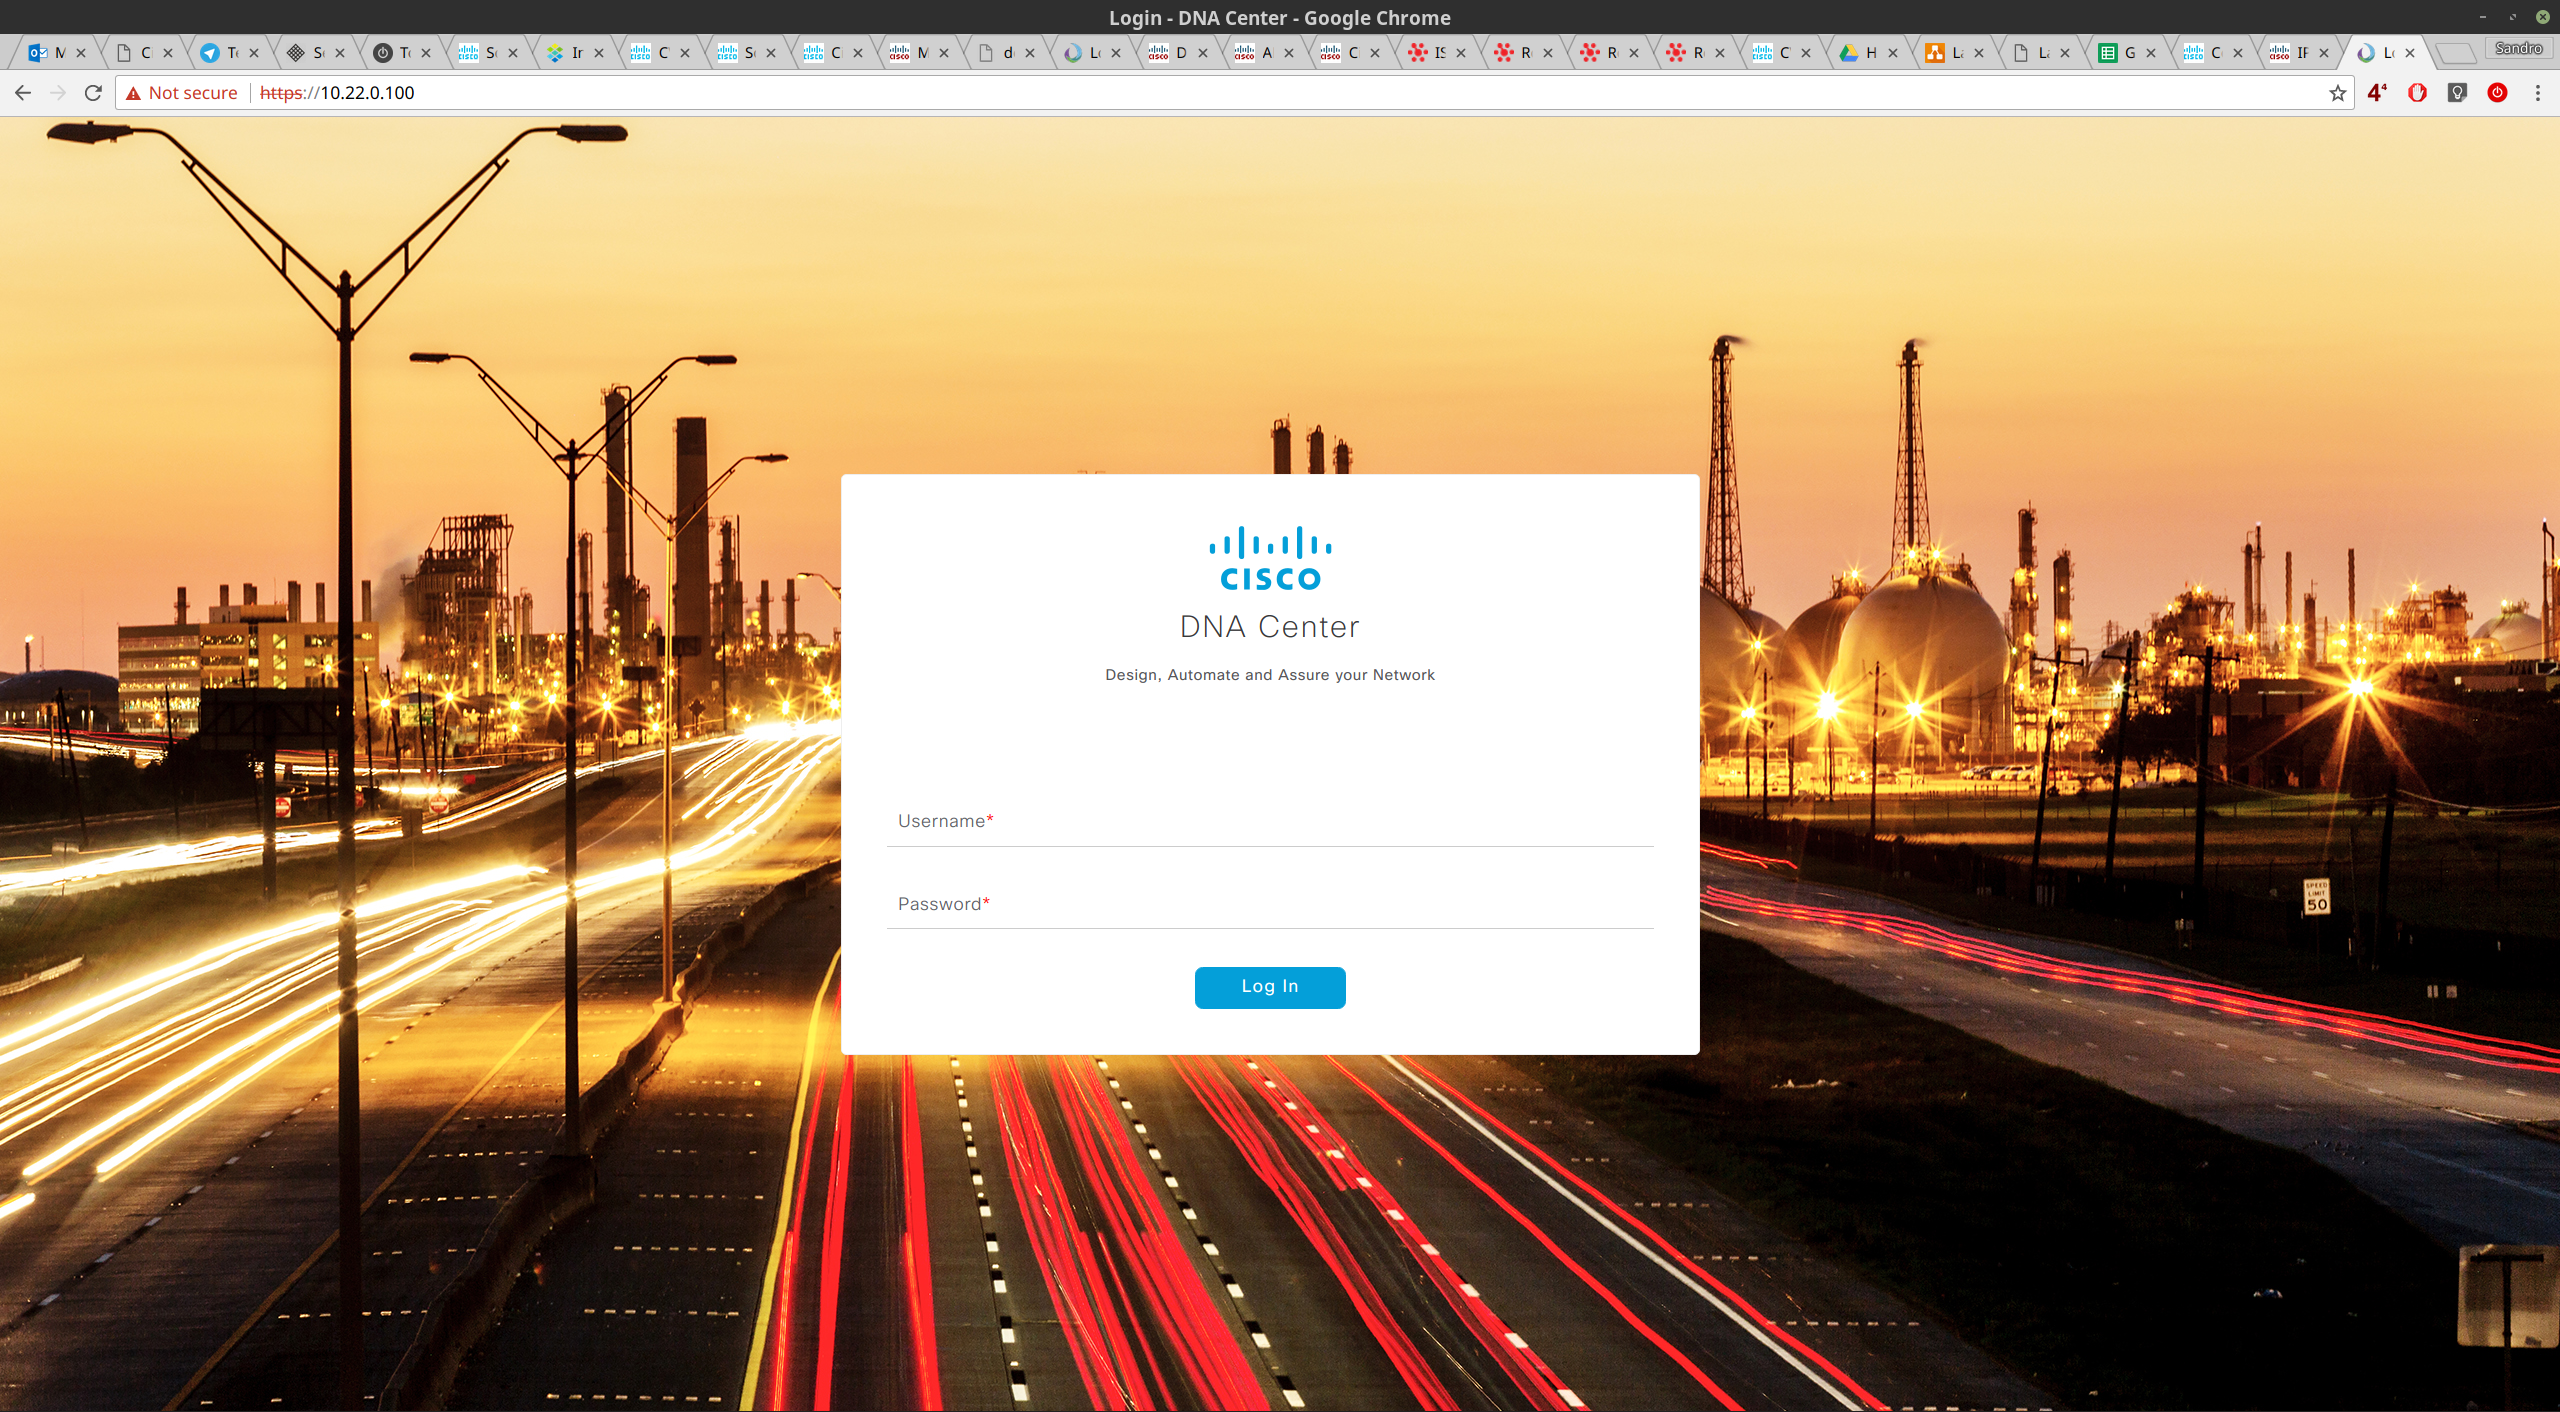
\includegraphics[height=9cm]{img/sc_005.png}
	\caption{DNA Center Web GUI - Loginpage}
	\label{fig:dna-center-gui-1}
\end{figure}

Gleich zu Begin verlangt das DNA Center die Cisco Credentials die mit dem Smart Account verknüpft sind, die die Lizenzen verwaltet. Dieser Schritt kann übersprungen werden. 

\begin{figure}[H]
	\centering
	\includegraphics[height=9cm]{img/sc_006.png}
	\caption{DNA Center Web GUI - Cisco Credentials for Licences}
	\label{fig:dna-center-gui-2}
\end{figure}

Der IPAM Server (in unserem Fall Infoblox) wird auch gleich zu beginn verlangt. Auch dieser Schritt kann vorerst übersprungen werden.

\begin{figure}[H]
	\centering
	\includegraphics[height=9cm]{img/sc_007.png}
	\caption{DNA Center Web GUI - Cisco IPAM}
	\label{fig:dna-center-gui-3}
\end{figure}

\begin{figure}[H]
	\centering
	\includegraphics[height=9cm]{img/sc_008.png}
	\caption{DNA Center Web GUI - Dashboard}
	\label{fig:dna-center-gui-4}
\end{figure}

\subsection{DNA Center Updates}

Der Updateprozess bringt einige Hürden mit sich:
\begin{itemize}
	\item System Updates müssen vor den Package Updates installiert werden.
	\item Werden die Package Updates vor dem System Update ausgeführt, können diese blockieren. 
	\item Die Package Updates müssen in der richten Reihenfolge installiert werden.
	\item Die oben genannte Reihenfolge ist nicht direkt ersichtlich.
	\item Der Updatevorgang dauert mehrere Stunden.
	\item Der Updatefortschritt wird nicht angezeigt. 
	\item Während dem Updateprozess können Teile des Web-GUIs Fehlermeldungen anzeigen oder überhaupt nicht mehr erreichbar sein.
\end{itemize}

Folgende Ansicht ist unter Einstellungen (Zahnrad-Symbol) => Management zu finden:

\begin{figure}[H]
	\centering
	\includegraphics[width=\columnwidth]{img/sc_009.png}
	\caption{DNA Center App Management}
	\label{fig:dna-center-gui-update-1}
\end{figure}

Abgestürzte Packete können mit den folgenden Befehlen wieder restauriert werden (Am Beispiel von main-system-package:1.0.4.779):

\begin{lstlisting}[language=bash]
$ maglev package status | awk  '$3 ~ /[0-9]+/ {print $1":"$3}'| grep -v "^system" |  while read pkg; do maglev catalog package delete $pkg;done
$ maglev system_update_package install main-system-package:1.0.4.779
\end{lstlisting}

Nach einem Update wurde die Reihenfolge von System und Package Update angepasst. Vermutlich um den Administrator dazu zu bringen zuerst die System Updates zu installieren. 

\begin{figure}[H]
	\centering
	\includegraphics[height=4cm]{img/sc_010.png}
	\caption{DNA Center App Management - Alte Menü Anordnung}
	\label{fig:dna-center-gui-update-2}
\end{figure}

\subsubsection{Schwierigkeit: Cisco CCO Login für Updates notwendig}

Application Packages und Updats können nur Installiert werden, wenn die Cisco CCO Credentials hinterlegt sind.

\begin{figure}[H]
	\centering
	\includegraphics[height=4cm]{img/dan-center-cisco-credentials-required.png}
	\caption{DNA Center Upgrade - Cisco Credentials required}
	\label{fig:dna-center-cisco-credentials-required}
\end{figure}

\subsubsection{Schwierigkeit: Unterschiedliche Versionsangabe}

Beim Updatevorgang kann es zu Verwirrungen kommen, weil die Versionangabe von der Funktion About von der Version des System Packages abweicht.

\begin{figure}[H]
	\centering
	\includegraphics[height=3cm]{img/dna-center-about.png}
	\caption{DNA Center - About - Version}
	\label{fig:dna-center-about}
\end{figure}

\begin{figure}[H]
	\centering
	\includegraphics[height=2.5cm]{img/dna-center-system-upgrade-version.png}
	\caption{DNA Center - System Upgrade - Version}
	\label{fig:dna-center-system-upgrade}
\end{figure}

\subsection{Cisco PNP mit DNA Center}

\paragraph{DHCP Konfiguration}

\begin{itemize}
	\item DNA Center akzeptiert Cisco PNP Anfragen via http
	\item Cisco Switches/Router versuchen beim ersten Boot ohne Konfiguration DHCP zu machen und Cisco PNP
\end{itemize}

Die Cisco PNP Discovery kann über die DHCP Optione 43 und 60 konfiguriert werden (Siehe \cite{cisco-pnp-dhcp}). In unserem Fall haben wir diese Optionen auf dem Infoblox konfiguriert.

\begin{figure}[H]
	\centering
	\includegraphics[height=10cm]{img/Infoblox_PNP.png}
	\caption{Infoblox Cisco PNP DHCP Option Konfiguration}
	\label{fig:cisco-pnp}
\end{figure}

\subsection{Automatischer "Claim" von Netzwerkgeräten}

\subsubsection{DNA Center Provision - Unclaimed Devices}

Nachdem die DHCP Option erfolgreich konfiguriert ist, erscheinen die Geräte im Device Inventory.

\begin{figure}[H]
	\centering
	\includegraphics[height=8cm]{img/DNA_Center_All_Fabric2_Unclaimed.PNG}
	\caption{DNA Center Provision - Alle Geräte erfolgreich in der "Unclaimed List"}
	\label{fig:dna-center-provision-unclaimed}
\end{figure}

Bevor es jedoch so weit kam, wurden verschiedene Fehlermeldungen angezeigt. Diese konnten jeweils behoben werden indem das betroffene Gerät auf Werkeinstellung zurückgesetzt und neu gestartet wurde. Dieser Vorgang wurde so lange wiederholt bis keine Fehlermeldungen mehr angezeigt wurden. 

\begin{figure}[H]
	\centering
	\includegraphics[height=4cm]{img/DNA_Center_Unclaimed_Errors_1.PNG}
	\caption{DNA Center Provision - Fehlermeldungen in der "Unclaimed List"}
	\label{fig:dna-center-provision-unclaimed-2}
\end{figure}

\subsection{DNA Center Netzwerk Design}

\subsubsection{Network Hierarchy}

Gemäss unserem \ref{fig:LabNetworkArchitecture} haben wir zwei Standorte. Rapperswil mit zwei Gebäuden und Jona mit einem Gebäude.
In DNA Center können diese sehr einfach im Abschnitt Design => Network Hierarchy hinzugefügt werden.

\begin{figure}[H]
	\centering
	\includegraphics[height=8cm]{img/Selection_011.png}
	\caption{DNA Center Design Map}
	\label{fig:dna-center-design-1}
\end{figure}

\begin{figure}[H]
	\centering
	\includegraphics[height=6cm]{img/Selection_012.png}
	\caption{DNA Center Design - Standort hinzufügen}
	\label{fig:dna-center-design-2}
\end{figure}

\begin{figure}[H]
	\centering
	\includegraphics[height=6cm]{img/Selection_014.png}
	\caption{DNA Center Design - Gebäude können mit Koordinaten hinzugefügt werden.}
	\label{fig:dna-center-design-3}
\end{figure}

\begin{figure}[H]
	\centering
	\includegraphics[height=8cm]{img/design_map_overview.PNG}
	\caption{DNA Center Design - Übersicht über alle Standorte und Gebäude}
	\label{fig:dna-center-design-overview}
\end{figure}

\subsection{Manuelle Underlay Konfiguration mit ISIS}
Da die automatische Erstellung des Underlay Netzwerkes nicht funktionierte, mussten wir es selber Konfigurieren. 

\subsubsection{Script Automation}

\subsubsection{ISIS}

\subsection{Netzwerkgeräte zu Inventory hinzufügen}


\subsection{Manuel Geräte im DNA Center hinzufügen}
Da alle Versuche die Geräte automatisch hinzuzufügen gescheitert sind, entschieden wir uns den Vorgang manuell Durchzuführen. 

Im Dashboard klickt man dazu auf Inventory (Siehe \ref{fig:dna-center-inventory-button})

\begin{figure}[H]
	\centering
	\includegraphics[height=3cm]{img/dna-center-inventory-button.PNG}
	\caption{DNA Center Dashboard - Inventory Knopf}
	\label{fig:dna-center-inventory-button}
\end{figure}

Anschliessend wählt man "Add" (siehe \ref{fig:dna-center-inventory-add})

\begin{figure}[H]
	\centering
	\includegraphics[height=3cm]{img/dna-center-inventory-add.PNG}
	\caption{DNA Center Inventory - Gerät hinzufügen}
	\label{fig:dna-center-inventory-add}
\end{figure}

Anschliessend müssen folgende Informationen eingegeben werden:
\begin{itemize}
	\item Device Type
	\item Device IP \ Name
	\item SNMP (Version, Read und Write Community)
	\item CLI (via SSH oder Telnet) \textit{oder}
	\item NETCONF
\end{itemize}

Wir entschieden uns CLI via SSH zu nehmen. Von NETCONF und CLI muss nur eine von beiden Optionen gewählt werden. 

\begin{figure}[H]
	\centering
	\includegraphics[height=5cm]{img/dna-center-inventory-add-form.png}
	\caption{DNA Center Inventory - Formular Gerät hinzufügen}
	\label{fig:dna-center-inventory-add-form}
\end{figure}

Danach erscheint das Gerät in der Liste (Siehe \ref{fig:dna-center-inventory-index-new})

\begin{figure}[H]
	\centering
	\includegraphics[height=2cm]{img/dna-center-inventory-index-new.png}
	\caption{DNA Center Inventory - Neue Geräte in der Liste}
	\label{fig:dna-center-inventory-index-new}
\end{figure}

TBA: Neue Images herunterladen und mit Golden Tag versehen. 

\subsection{Image Repository}
Im DNA Center können Netzwerkgeräte automatisch geupdatet werden. Sobald ein Gerät im Inventory erfolgreich hinzugefügt worden ist, sucht das DNA Center nach Updates. Die Verfügbaren Images sind unter Desing => Global => Image Repository zu finden.

\begin{figure}[H]
	\centering
	\includegraphics[height=2cm]{img/dna-center-design-image-repository.png}
	\caption{DNA Center Design - Image Respository}
	\label{fig:dna-center-design-image-repository}
\end{figure}

\subsection{Automatisches Softwareupdate von Netzwerkgeräten}

Im DNA Center besteht die Möglichkeit bei "claimed Devices" ein automatisches Softwareupdate durchzuführen. Dies hat bei keinen von unseren Switches oder Routern geklappt. 

\begin{tabular}{ | l | l |}
	\hline
	\textbf{Methode} & \textbf{Resultat} \\
	\hline	
	\makecell{via DNA Center \\ \textit{nutzt HTTP \& SFTP}} & Fehlgeschlagen (Siehe \ref{fig:dna-center-provision-updates-1}) \\
	CLI - HTTPS    & Fehlgeschlagen (Siehe \ref{fig:dna-center-provision-updates-2}) \\
	CLI - SCP      & Fehlgeschlagen (Siehe \ref{fig:dna-center-provision-updates-3}) \\
	CLI - TFTP     & Erfolgreich (Siehe \ref{fig:dna-center-provision-updates-4}) \\	
	\hline	
\end{tabular}
\captionof{table}{Softwareupdate - Übersicht Methoden und ausgeführten Versuche}

\begin{figure}[H]
	\centering
	\includegraphics[height=8cm]{img/updates/Selection_070.png}
	\caption{DNA Center Provision - Nachdem manuellen hinzufügen, muss die Firmware aktualisiert werden.}
	\label{fig:dna-center-provision-updates}
\end{figure}


\begin{figure}[H]
	\centering
	\includegraphics[height=5cm]{img/updates/Selection_071.png}
	\caption{Fehlermeldung Updatevorgang via DNA Center}
	\label{fig:dna-center-provision-updates-1}
\end{figure}

\subsection{Manuelles Softwareupdate via separaten TFTP Server}
Weil das automatische Update nicht funktioniert hat, mussten wir die Images manuell auf die Switches und Router aufspielen.

\begin{figure}[H]
	\centering
	\includegraphics[height=2cm]{img/updates/Selection_082.png}
	\caption{Firmwareupdate Switch via CLI HTTPs}
	\label{fig:dna-center-provision-updates-2}
\end{figure}

\begin{figure}[H]
	\centering
	\includegraphics[height=5cm]{img/updates/Selection_108.png}
	\caption{Firmwareupdate Switch via CLI SCP}
	\label{fig:dna-center-provision-updates-3}
\end{figure}

\begin{figure}[H]
	\centering
	\includegraphics[height=2cm]{img/updates/Selection_111.png}
	\caption{Firmwareupdate Switch via CLI TFTP}
	\label{fig:dna-center-provision-updates-4}
\end{figure}

\subsection{Lizenzen}
Die Lizenzen bezieht das DNA Center automatisch von den Cisco Server. 
\begin{figure}[H]
	\centering
	\includegraphics[height=3cm]{img/LicenceManager_001.png}
	\caption{Der Licence Manager ist über das Dashboard erreichbar.}
	\label{fig:dna-center-licence-1}
\end{figure}

\begin{figure}[H]
	\centering
	\includegraphics[height=6cm]{img/Selection_006.png}
	\caption{Ohne Verlinkten CSSM Account können keine Lizenzen zugewiesen werden.}
	\label{fig:dna-center-licence-3}
\end{figure}

\begin{figure}[H]
	\centering
	\includegraphics[height=6cm]{img/Selection_008.png}
	\caption{Der im DNA Center hinterlegte Cisco Account muss Zugriff zum entsprechenden Smart Account haben.}
	\label{fig:dna-center-licence-4}
\end{figure}

\begin{figure}[H]
	\centering
	\includegraphics[height=5cm]{img/LicenceManager_002.png}
	\caption{Der korrekt hinterlegte Account}
	\label{fig:dna-center-licence-5}
\end{figure}

\begin{figure}[H]
	\centering
	\includegraphics[height=8cm]{img/LicenceManager_003.png}
	\caption{Übersicht über die den Netzwerkkomponeten zugewiesenen Lizenzen}
	\label{fig:dna-center-licence-6}
\end{figure}

\begin{figure}[H]
	\centering
	\includegraphics[height=6cm]{img/LicenceManager_004.png}
	\caption{Nicht jedem Gerät kann eine Lizenz gewiesen werden. (Siehe Tabelle)}
	\label{fig:dna-center-licence-7}
\end{figure}

\begin{tabular}{ | c | c | }
	\textbf{Geräteserie} & 	\textbf{Lizenzzuweisung möglich} \\
	\hline
	Cisco Catalyst 9300 Series Switches & Ja \\
	Cisco Catalyst 3850 Series Ethernet Stackable Switch & Ja \\
	Cisco 4400 Series Integrated Services Routers & Nein \\
\end{tabular}

\subsection{Device Provisioning via DNA Center}
Um den einzelnen Netzwerkgeräten einen Namen und die Basis Konfiguration zu geben, wird im DNA Center unter \textit{Provision -> Devices} die zu provisionierende Geräte ausgewählt. Danach wird \textit{Action -> Provision Device} der Provision Vorgang gestartet.

Dazu muss zuerst im Template Editor ein Template hinzugefügt werden.

TBA: Template Editor Screenshots


\subsection{Overlay Provisioning via DNA Center}


\subsection{BGP über Legacy Netzwerk}

Für das Overlay Provisioning verwendet das DNA Center BGP. Dabei ist uns aufgefallen das die Cisco Catalyst 3850 Series Switche nur eine Lizenz für IP Base installiert haben und BGP nur in der IP Services Lizenz unterstützt wird. Die genauen Unterschiedene der verschiedenen IOS Software Features sind in untenstehender Grafik ersichtlich\cite{cisco-3850-faq}:

\begin{figure}[H]
	\centering
	\includegraphics[width=16cm]{img/IPBaseServices.png}
	\caption{IP Base and Services}
	\label{fig:IP Base and Services}
\end{figure}

Über die CLI konnten konnten wir eine IP Services Evaluation Lizenz für 90 Tage aktivieren.

\begin{lstlisting}[language=bash]
sh license right-to-use activate ipservices all accepptEULA
reload
show license right-to-use
\end{lstlisting}

\subsection{Fabric Konfigurieren}
Nach der manuellen Konfiguration des Underlays, dem hinzufügen der Geräte, dem Update und dem Provisionieren, konnten wir endlich die Fabric konfigurieren. 

Erreichbar ist das unter \textit{Provision -> Fabric}. Nachfolgend wir der entsprechende Standort ausgewählt.

Den einzelnen Netzwerkgeräten werden nun mit Rechtsklick folgende Rollen zugeteilt:
\begin{itemize}
	\item Border
	\item Border + CP (Control Plane)
	\item Edge
\end{itemize}

Nachdem alle Geräte der entsprechenden Fabric zugeteilt worden sind, kann die Konfiguration gespeichert und wird auf die Geräte geschrieben. 

\begin{figure}[H]
	\centering
	\includegraphics[width=16cm]{img/dna-center-fabric-1.png}
	\caption{DNA Center Provision - Fabric - Nach der Zuteilung wird die Konfiguration auf die Geräte geschrieben.}
	\label{fig:IP Base and Services}
\end{figure}


\begin{tabular}{| l | l | l | l | l |}
	\textbf{Darstellung} & \makecell{\textbf{Teil der}\\ \textbf{Fabric}} & \makecell{\textbf{Änderung}\\ \textbf{ausstehend}} & \textbf{Provisioniert} & \textbf{Bemerkung} \\
	\hline
	Grau & Ja & Nein & Nein & \\
	Schwarz & Nein & Nein & Nein & \\
	Grau mit blauem Rand & Ja & Ja & Nein & \\
	Blau & Ja & Nein & Ja & \\
	Umrandung mit Pfeil & - & - & - & Gruppierte Geräte\\	

\end{tabular}
\captionof{table}{DNA Center Provision - Fabric - Darstellung}

\subsection{Policies definieren}
Damit die Fabric Konfiguriert werden kann, müssen folgende Bedienungen erfüllt sein:





\subsection{Cisco ISE Verknüpfen und Gruppen anlegen}

\subsection{Ping zwischen zwei Clients}

\subsection{DNA Center Reset}
Da nach einigen Versuchen weder ein funktionsfähiges Under- noch Overlay Netzwerk vorhanden war, hatten wir uns entschieden das DNA Center neu zu Konfigurieren.

\begin{lstlisting}[language=bash]
$ maglev-config-wizard #DO NOT EXECUTE THIS COMMAND
\end{lstlisting}

Als folge dieses Befehls, nachdem alle Parameter eingegeben wurden, kam die folgende Meldung:

\begin{figure}[H]
	\centering
	\includegraphics[height=10cm]{img/dna-center-reset-fail-1.png}
	\caption{DNA Center - maglev-config-wizard - Fehlermeldung}
	\label{fig:dna-center-reset-1}
\end{figure}

Nach einem Neustart der Appliance kam die folgende Meldung und das System bootete nicht mehr. 
\begin{figure}[H]
	\centering
	\includegraphics[height=1cm]{img/dna-center-reset-fail-2.png}
	\caption{DNA Center - Boot Fehlermeldung}
	\label{fig:dna-center-reset-2}
\end{figure}

In der Anleitung wird dieser Befehl so nicht erwähnt. Bei einem früheren Versuch diesen Befehl auszuführen, um den NTP Server zu ändern, führte es jedoch nicht zu diesem Fehler. 

\paragraph{Neuinstallation}
In folge war es notwendig die Cisco DNA Center Appliance neu zu installieren. 

\begin{figure}[H]
	\centering
	\includegraphics[height=2cm]{img/dna-center-reset-iso.png}
	\caption{DNA Center - Neuinstallation - Installations ISO wird auf USB Drive kopiert}
	\label{fig:dna-center-iso-1}
\end{figure}

Das USB Drive wird direkt in die Appliance gesteckt und gebootet. Der weitere Installationsprozess sieht aus wie im Abschnitt \ref{DNACenterSetup_Installation} gezeigt. 

\alertwarningbox{
	Nach der Neuinstallation sind alle Daten und die Konfiguration gelöscht. Eine Option die Konfiguration beizubehalten gibt es nicht.
}

\subsection{Zweiter Versuch}
Im ersten Versuch haben wir die LAN Automation übersprungen. Das stellt jedoch einer der wichtigen Features des DNA Centers dar. Mit der Unterstützung von Patrick Mosimann sind wir alles Schritt für Schritt durchgegangen. 

\subsection{DNA Center Netzwerk Design}
Wie im ersten Teil

\subsection{Alle Netzwerkkomponenten vorgehen}

\subsection{ISE reset}

\subsection{Credentials korrekt hinterlegen}

\subsection{Fabric Border - Seeddevice}

\subsection{ISE Integration}

\subsection{Netzwork Discovery - LAN Automation}

